\chapter{Anforderungsanalyse und Konzept}\label{chap:Konzept}
Dieses Kapitel befasst sich mit der Konzeptentwicklung für die Anwendung und den zu entwickelnden Prototyp. Dazu wurden verschiedene Anwendungsfälle betrachtet und spezifische Anforderungen erhoben.

\section{Die Idee}
Die Hauptzielgruppe der Anwendung ist der Bildungsbereich. Sie soll Schülern, Studieren und auch Professoren die Möglichkeit bieten mit Hilfe von Augmented Reality das Lernen sowie Lehren zu bereichern. \\
Das Grundprinzip ist dabei folgendes: Die App soll dem Anwender die Möglichkeit geben 3D-Modelle hochzuladen, für die dann ein einzigartiger Marker generiert wird. Dieser kann dann ausgedruckt oder anderweitig angezeigt werden. Mit Hilfe der Kamera lässt sich dann das entsprechende 3D-Modell im Augmented Reality Bereich darstellen.

\section{Mögliche Anwendungsfälle}
Im folgenden werden ein paar mögliche Anwendungsfälle für verschiedene Personen definiert.

\subsection{Der Professor}
Das Anwendungsszenario, welches für einen Professor oder Lehrer denkbar wäre, orientiert sich an der bereits existierenden Webseite Socrative,\todo{ref socrative} welche bereits im Universitätsalltag häufig eingesetzt wird und Lehrenden die Möglichkeit gibt Umfragen zu erstellen, die von Studierenden über einen Raumcode beantwortet werden können. \\
Ein solches Raumsystem wäre auch für die AR Anwendung denkbar.
Mit Hilfe der Anwendung könnte dann ein Professor einen Raum erstellen, in welchem er verschiedene 3D-Modelle speichern könnte, die Marker könnten im Anschluss dann Online zur Verfügung gestellt, über Ausdrucke vervielfältigt oder in die Präsentation eingebunden werden.\\
Die Studierenden können dann über einen Zugangscode dem Raum beitreten und dann mit Hilfe der Kamera die  entsprechenden Modelle des Raumes, in dem sie sich aktuell befinden, anzeigen lassen.

\subsection{Die Studierenden}\label{sec:Anwendungsfall:Studierender}
Den Studierenden soll neben der Möglichkeit öffentlichen Räumen beizutreten auch die Möglichkeit gegeben werden selbst Modelle hochzuladen und die entsprechenden Marker zum Beispiel auf Lernzettel zu drucken. Dazu könnte jeder einen privaten Raum besitzen. Die Modelle die der Anwender hier hochlädt, wären dann nur lokal gespeichert und nicht öffentlich über einen Code oder Ähnlichem zugänglich. 

\section{Der Prototyp}
Der zu entwickelnde Prototyp fokussiert sich dabei auf die Umsetzung der Augmented Reality und das Erstellen der zu Trackenden Marker. Die Modelle die hochladen werden dabei lediglich lokal gespeichert. \\
Dadurch handelt es sich bei dem Prototyp um eine Umsetzung des \glqq privaten Raumes\grqq . Er bietet dem Anwender nicht die Möglichkeit die Modelle zuteilen.\\ 
Eine ansonsten notwendige Datenspeicherung auf einem Server, das Implementieren eines Raumsystems mit Zugangscode und weitere Funktionen fallen dadurch bei diesem ersten Prototyp weg.


\section{Anforderungsanalyse}\label{sec:Anforderungsanalyse}
Im folgenden wird eine Anforderungsanalyse für den zu entwickelnden Prototyp durchgeführt.

\subsection{Kontext des Prototyps}
Die Anwendung besteht aus drei Unterfunktionen dem Generieren von Markern, dem Tracken von Markern und dem Rendern von Modellen.\\
Die generierten Marker benötigen dabei alle eine unterschiedliche ID, um im Anschluss beim Tracking unterschieden werden zu können. Außerdem müssen sie aus jeder Rotation eindeutig zuerkennen sein. Dafür müssen sich zwei Marker auch unterscheiden, wenn einer von ihnen beliebig rotiert wurde.\\
Um beim Rendern das Modell realistisch in Relation zum Marker zu platzieren, werden die Position, Rotation, Größe und Transformation des Markers benötigt. \todo{überarbeiten}


\subsection{Anwendungsfälle des Prototyps}
Ein beispielhaftes Anwendungsszenario des Prototypen, das sich aus dem Anwendungsfall des Studierenden ableitet (siehe Abschnitt \ref{sec:Anwendungsfall:Studierender}), ist die mit dem Prototyp generierten Marker auf einem Lernzettel einzufügen und ein vorlesungsrelevantes Modell zu verlinken. Dazu wird das Modell in dem Prototyp hochgeladen und der generierte Marker in ein Dokument eingefügt. Im Anschluss kann dann das Dokument mit der Kamera gefilmt werden, um das 3D-Modell anzeigen zu lassen.\todo{Weiterer Anwendungsfall?}\\
Die folgende Abbildung \ref{fig:Use-Cases} zeigt eine Zusammenfassung der Funkionen des Prototyps in einem Anwendungsfalldiagramm.
\begin{figure}[h!]
\centering
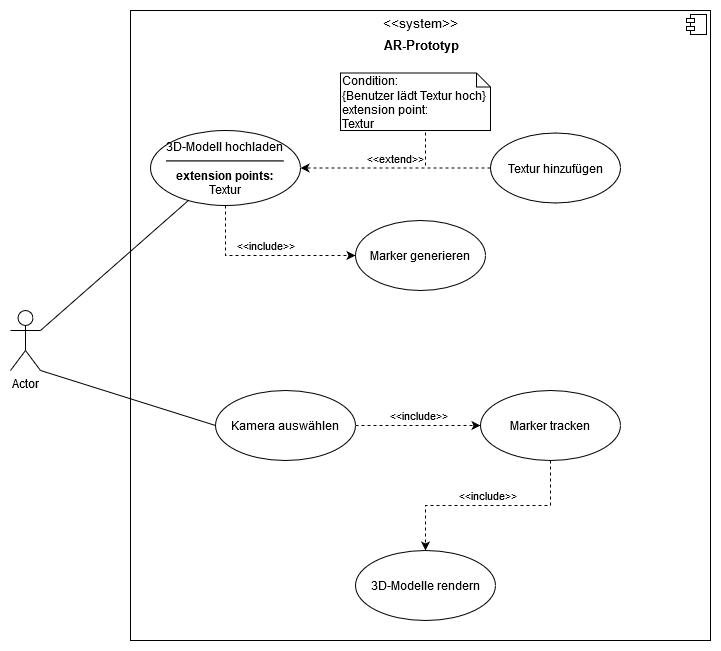
\includegraphics[width=1.0\textwidth]{Abbildungen/Use-Case-Diagramm.png}
\caption[Use Cases des Prototyps]{Use Case Diagramm des Prototyps. (Quelle: Eigene Darstellung)}
\label{fig:Use-Cases}
\end{figure}

\subsection{Anforderungen an den Prototyp}
Im folgenden Abschnitt werden aus den Anwendungsfällen funktionale und nichtfunktionale Anforderungen abgeleitet. 
\subsubsection{Funktionale Anforderungen}
\begin{itemize}
\item Das System soll auf einem Android Smartphone laufen.
\item Der Benutzer soll eigene 3D-Modelle als OBJ-Dateien hochladen können.
\item Die Anwendung soll 3D-Modelle im Kamerabild anzeigen können.




\end{itemize}

\subsubsection{Nichtfunktionale Anforderungen}
\begin{itemize}
\item Das Tracking soll mit 30FPS laufen.
\item Das Tracking soll bei vollständig erkanntem Marker robust gegenüber Rotation, Skalierung, Perspektive und Belichtung sein.

\item Die Anwendung soll in Android Studio entwicklet werden.
\item Als Programmiersprache soll Java verwendet werden.

\item Das Tracking soll mittels eines markerbasierten Verfahrens realisiert werden.
\item Das System soll ein Set an Markern erkennen und unterscheiden können.

\item Die Anwendung soll OBJ-Datei laden und verarbeiten können.
\item Das System soll Textur-Dateien im Bildformat(jpeg, png) laden und verarbeiten können.





\end{itemize}
\section{Konzept des Prototyps}



